\documentclass[notitlepage]{mcmthesis}
%\renewcommand\appendix{\setcounter{secnumdepth}{-2}}
\mcmsetup{tcn= 87207, problem = E,
    sheet = true, titleinsheet = false, keywordsinsheet = false,
    titlepage = false, abstract = false}
\setlength{\parskip}{0.1\baselineskip}
\usepackage{amsmath, amssymb, graphics, setspace}

\newcommand{\mathsym}[1]{{}}
\newcommand{\unicode}[1]{{}}
\newcommand{\tabincell}[2]{\begin{tabular}{@{}#1@{}}#2\end{tabular}}  
\setlength{\parindent}{0em}

\usepackage{palatino}
\usepackage{times}
\usepackage{verbatim}
\usepackage{graphicx}
\usepackage{subfigure}
\usepackage{multirow}
\usepackage{algorithmic}
%\usepackage[lined,algonl,boxed]{algorithm2e}
\usepackage{longtable}
\usepackage{array}
%\usepackage{subcaption}
\usepackage{stfloats}
\usepackage{balance}
\usepackage{multicol}
\usepackage{color}
\usepackage{epstopdf}
\usepackage{bm}
\usepackage{amsmath}
\usepackage{amssymb}
\usepackage{amsthm}
\usepackage{booktabs} % For formal tables
\usepackage{epsfig}
\usepackage{enumitem}
\usepackage{cleveref}
\usepackage{xspace}
\usepackage{url}
\usepackage{float}
%\usepackage{natbib}
\usepackage{booktabs}
\usepackage{makecell}
\usepackage{float}



\setlength\parskip{.8\baselineskip}
\setcounter{secnumdepth}{2}

\renewcommand{\algorithmicrequire}{\textbf{Input:}}   %Use Input in the format of Algorithm
\renewcommand{\algorithmicensure}{\textbf{Output:}}  %UseOutput in the format of Algorithm
\newcommand{\reminder}[1]{\textbf{\color{red}[** #1 **]}}  % to fix
\newcommand{\hide}[1]{} %hide
\newcommand{\vpara}[1]{\vspace{0.1in}\noindent\textbf{#1 }}
\newcommand{\para}[1]{\vspace{0.01in}\noindent\textbf{#1 }}
\newcommand{\secref}[1]{Section~\ref{#1}} %section reference
\newcommand{\Real}{\ensuremath{\mathbb{R}}}  % Real numbers
\newcommand{\figref}[1]{Figure~\ref{#1}} %section reference
\newcommand{\beq}[1]{\vspace{-0.01in}\begin{equation}#1\end{equation}\vspace{-0.01in}}
\newcommand{\beqn}[1]{\vspace{-0.01in}\begin{eqnarray}#1\end{eqnarray}\vspace{-0.01in}}
\newcommand{\besp}[1]{\begin{split}#1\end{split}}
\newcommand{\beal}[1]{\vspace{-0.03in}\begin{align}#1\end{align}\vspace{-0.03in}}

% Common mathematical notations
\DeclareMathOperator*{\argmax}{arg\,max}
\DeclareMathOperator*{\argmin}{arg\,min}
\DeclareMathOperator*{\diag}{diag}
\DeclareMathOperator*{\trace}{trace}
\newcommand\expt{\mathbb E}
\newcommand\prob{\mathbb P}
\newcommand\RR{\mathcal R}
% Specific Notations
\DeclareMathOperator*{\HFF}{\mathbf{H}} % human factor
%\DeclareMathOperator*{\EFF}{\mathbf{E}} % environmental factor
\DeclareMathOperator*{\EFF}{E}
\DeclareMathOperator*{\FFF}{\mathbf{F}} % fragility score
\DeclareMathOperator*{\FFS}{s_f}


\theoremstyle{definition}
\newtheorem{definition}{Definition}

\newtheorem*{remark}{Remark}
\newtheorem{theorem}{Theorem}

\newtheorem{eg}{Example}


\sloppy


\setkeys{Gin}{keepaspectratio, width=1 \textwidth}
\bibliographystyle{IEEEtran}
\title{
    A Human-oriented Merging Model for New Jersey}
\author{Bian Song}
\date{\today}
\begin{document}
    
    
    
    \begin{abstract}
        

    \end{abstract}
    
    \maketitle
    
    
    \begin{center}
        \textbf{\LARGE{A Refined Fragility Metric Based on Statistics}}
    \end{center}
    %\tableofcontents
    
    \setcounter{page}{1}


\section{Introduction}	

% introduction to topic.

% What is already done, and the gaps.
Quantifying the fragility of states based on human factors, such as the FSI score has been extensively studied by researchers and instutitions, such as in \reminder{cite some important works here. } However, these models does not consider the impact of environmental factors. For example, deterioation in natural environment may contribute on regional instability and violence~\reminder{some references required here}. As environmental factors are important in determining a state or a region's sustainability, merely considering human factors is clearly insufficient. 

% our work framework.
% some results.

% organization.
\section{Theoretical Framework}
\label{sec:model1}

\begin{figure}[t]
    \centering
   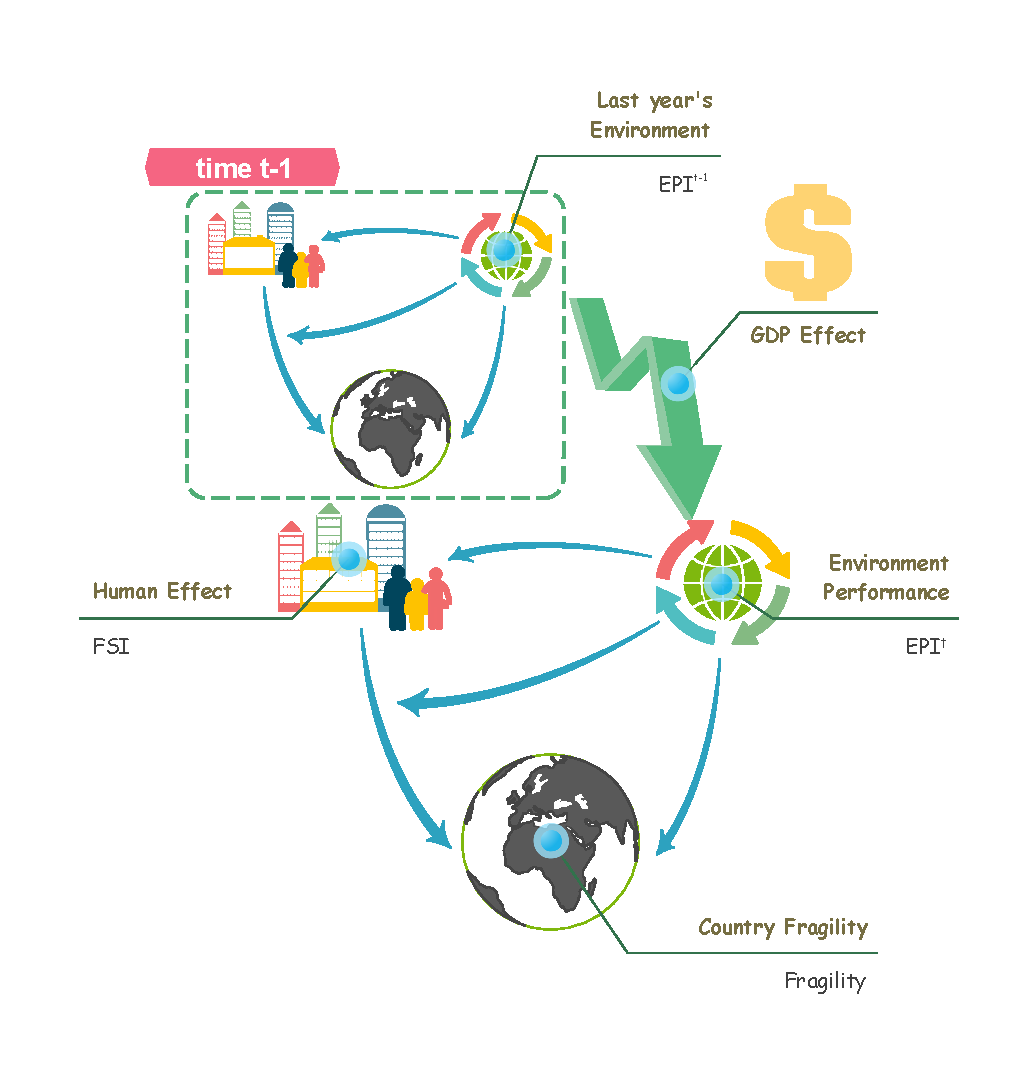
\includegraphics[width=.5\linewidth]{figs/model.eps} 
   \caption{Hypothesis Model Illustration}
   \label{fig:model:model}
\end{figure}

\begin{figure}[t]
   \centering
   \subfigure[Moderator variable model]{
       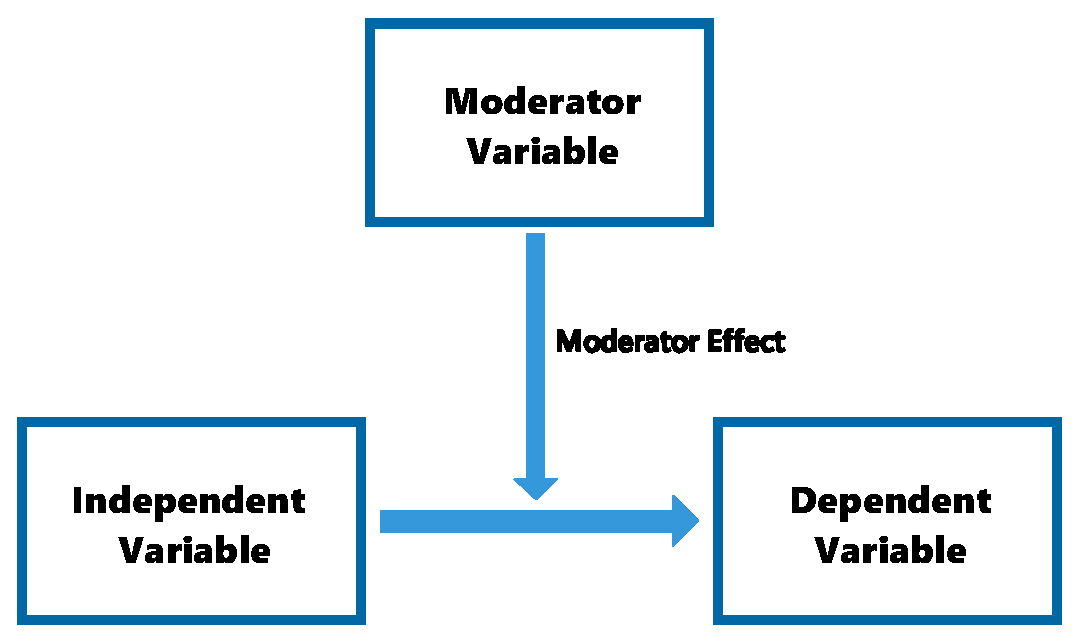
\includegraphics[width=.4\linewidth]{figs/model_moderator.eps}
       \label{fig:model:indirect:moderator}
   } 
   \subfigure[Mediator variable model]{
       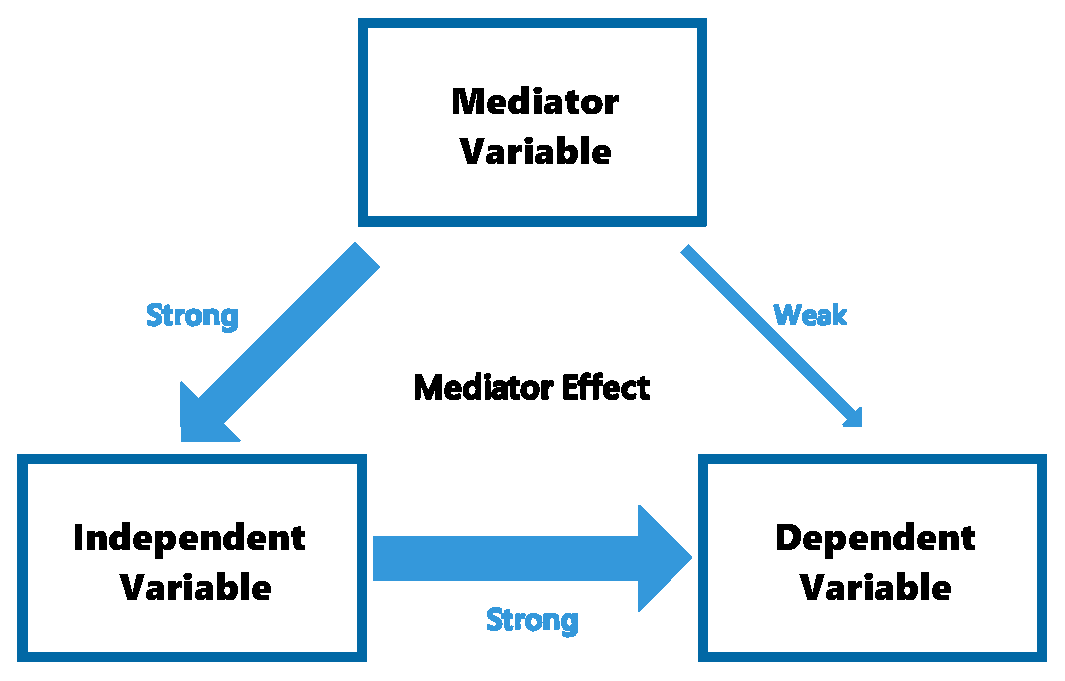
\includegraphics[width=.4\linewidth]{figs/model_mediator.eps}
       \label{fig:model:indirect:mediator}
   }
   %\label{fig:model:indirect}
   \caption{Hypothesis models for indirect effect of environmental factors. $\EFF$ represents environmental factors, $\HFF$ represents human factors, and $\FFF$ represents state fragility. The fragility is jointly determined by $\EFF$ and $\HFF$, by two hypothesis approach.}
\end{figure}
\label{sec:model}
In this part we propose theoretical framework for our analysis of the impact of climate change on \emph{state fragility}.
\subsection{Assumptions and Model Framework}
Our hypothesis framework is illustrated in Figure~\ref{fig:model:model}.
We propose two natural assumptions, based on which we derive the basic framework of our model. 
\begin{enumerate}
   \item The \emph{state fragility}, a concept to estimate the sustainability of states, is dependent on and only on \emph{human factors} and \emph{environmental factors.} \label{model:assump:1}
   \item The environmental factors and human factors interact with each other. \label{model:assump:2}
\end{enumerate}
The assumptions are natural. Assumption~\ref{model:assump:1} requires to quantify the fragility which considers both human factors and environmental factors. We propose a novel framework to quantify fragility by incorporating the human and environmental factors into a probabilistic framework.

Assumption~\ref{model:assump:2} requires a more sophisticated analysis of the two factors, including their respective and joint effects on the fragility, and the interaction between them. We are especially interested in the effects of environmental factors, which include \emph{direct} effect, which is the influence on fragility directly imposed by environmental factors; and \emph{indirect} effect, which is the influence on fragility imposed by envirionmental factors indirectly through human factors. Two hypothesis model to explain the indirect effect is visualized in Figure~\ref{fig:model:indirect:moderator} and~\ref{fig:model:indirect:mediator}.

The direct effect of environmental factors is measured by the effect of environmental factors on fragility score, with an unbiased estimation of the effect obtained by propensity score matching~\cite{caliendo2008some,dehejia2002propensity,hirano2004propensity}. The indirect effect of environmental factors can be explained by two hypothesis models: the \emph{moderator variable} model, as shown in Figure~\ref{fig:model:indirect:moderator}; and the \emph{mediator variable} model, as shown in Figure~\ref{fig:model:indirect:mediator}. We verify these two hypothesis.

In the following of this section, we are dedicated to enrich our model by developing several key ingredients: 
\begin{enumerate}
   \item A novel fragility score measure incorporating both environmental and human factors;
   \item The interaction pattern between human factors, envirionmental factors, and the fragility;
   \item The temporal model of a state's environmental status.
\end{enumerate}

The basic framework is sufficient to cover most of the requirements of the tasks.

\subsection{Representing the Two Factors}
\label{sec:model:rep}
\begin{table}[htbp]
   \centering
   \begin{tabular}{|c|c|} \hline 
      Notation & Description \\ \hline
      $\HFF $  & random variable of human factors \\ \hline
      $\EFF $ & random variable of environmental factors \\ \hline
      $ \FFF $ & binary random variable of fragility \\ \hline
      $\FFS $ & fragility score \\ \hline
   \end{tabular}
   \caption{Notations}
   \label{tab:model:notations}
\end{table}

\hide{
\begin{figure}[t]
    \centering
    \subfigure[FSI]{
        \includegraphics[width=.45\linewidth]{figs/fsi.eps}
        \label{fig:model:indexes:fsi}
    }
    \subfigure[EPI]{
        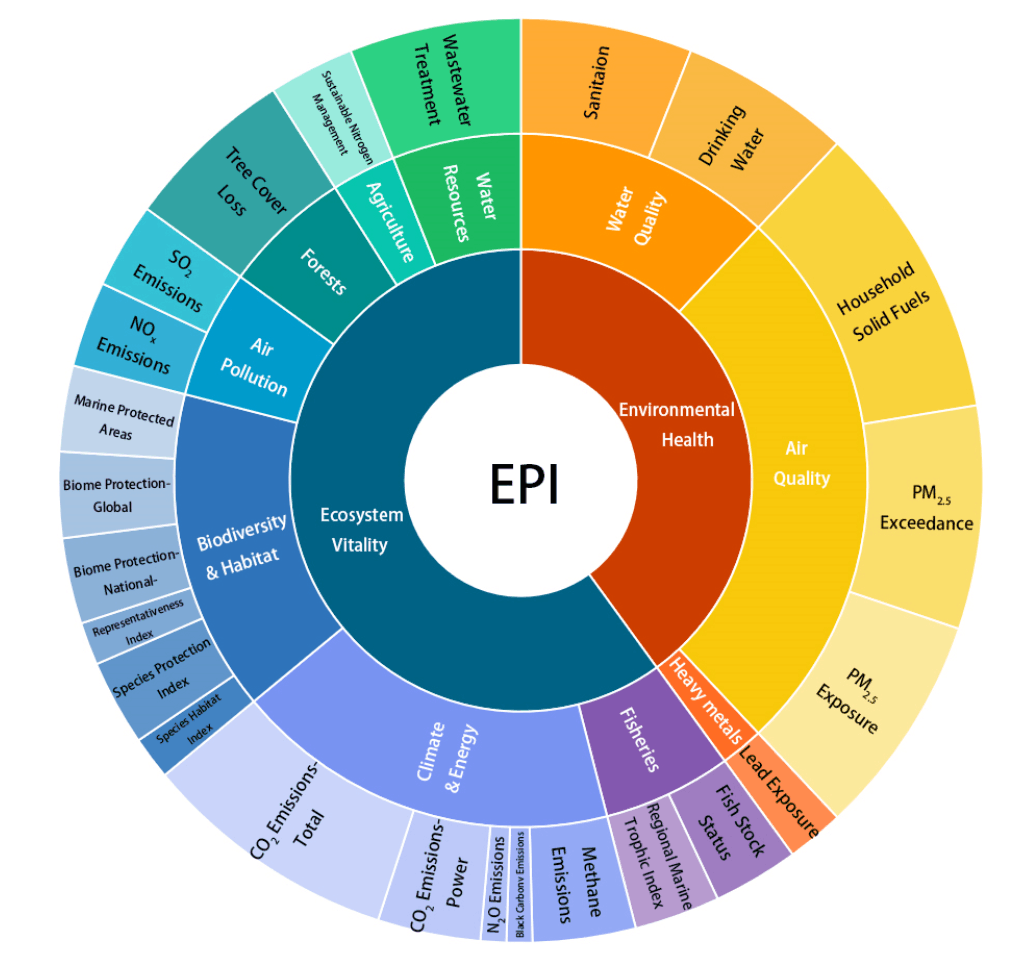
\includegraphics[width=.45\linewidth]{figs/epi.eps}
        \label{fig:model:indexes:epi}
    }
    \caption{The two fragiliy indexes.}
    \label{fig:model:indexes}
\end{figure}
}

\begin{figure}[htbp]
   \centering
   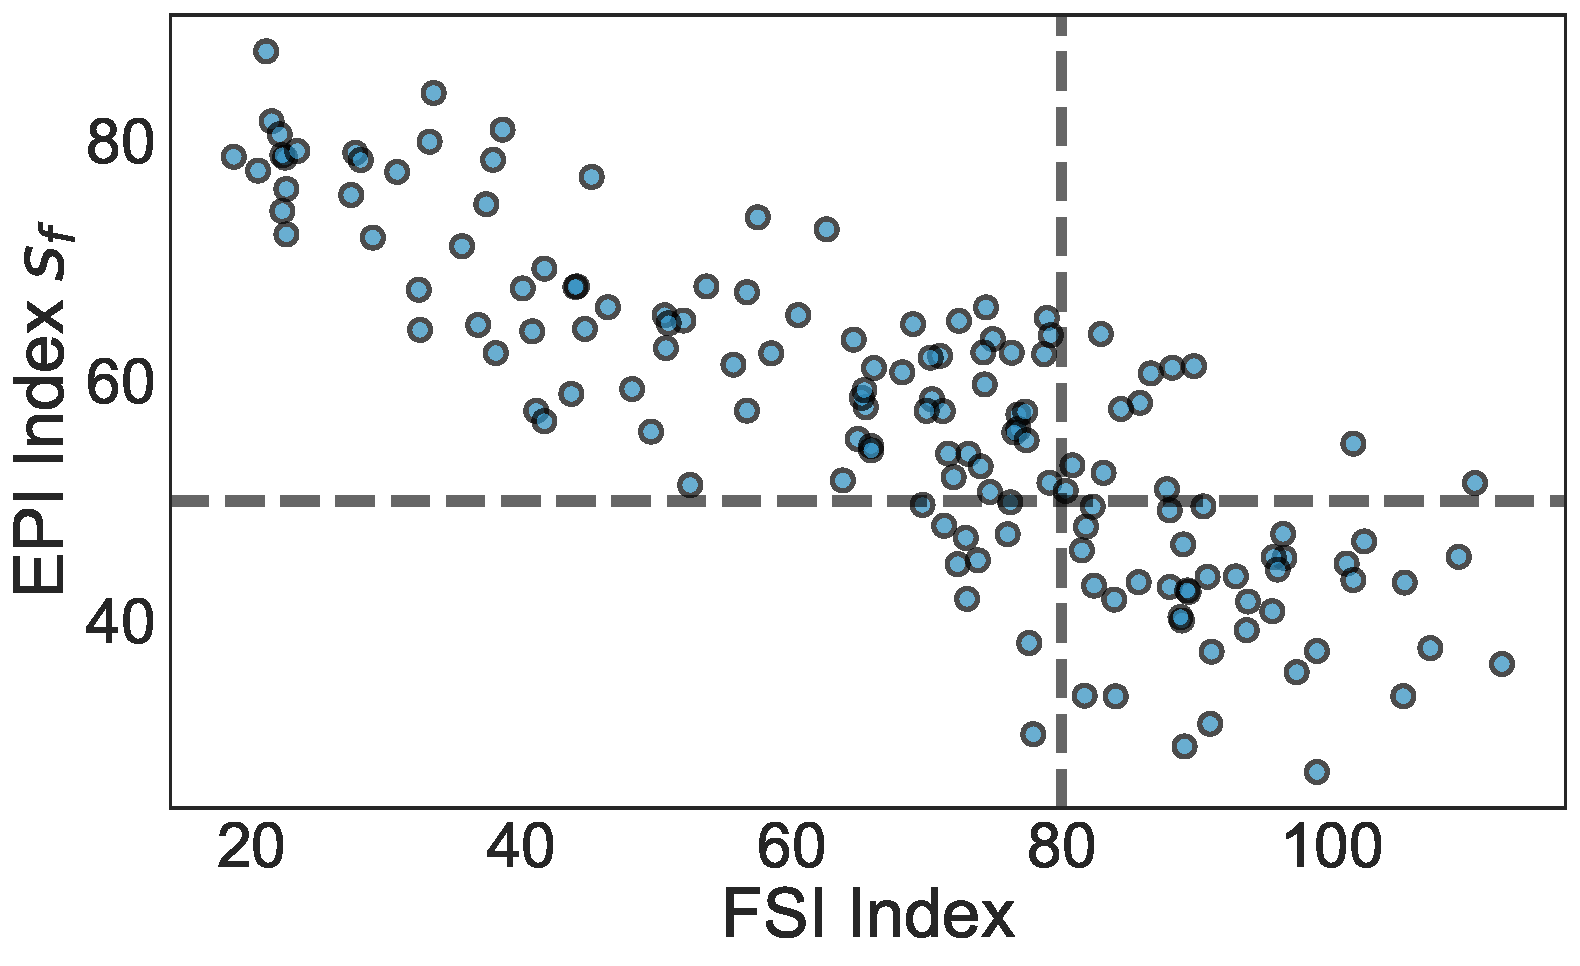
\includegraphics[width=.4\linewidth]{figs/fsiepi}
   \caption{EPI and FSI Indexes}
   \label{fig:model:epifsi}
\end{figure}

Basic notations are listed in Table~\ref{tab:model:notations}.
The variables in the table are theoretical. In order to reflect these variables numerically from empirical data, we introduce two widely recognized indexes:

\vpara{Environmental Performance Index (EPI).} It is an index to evaluate a state's environmental performance developed by Yale University~\cite{EPI_index}. It is composed of indicators in ecosystem vitality and environmental health. The higher the index, the better the environment, 

\vpara{Fragile States Index (FSI).} It is an index to measure a country's vulnerability to conflict developed by Fund for Peace and Foreign Policy by accounting for 12 social, economical, and political indicators.~\cite{FSI_index} Higher index indicates more vulnerability.

FSI index uses indicators relevant to human activity, and is therefore used as empirical data for $\HFF$. 
EPI index measures environmental fragility, and is therefore used as empirical data for $\EFF$.

Sometimes, we use binarized values of EPI and FSI indexes to denote the status of a state. The threshold and the relation between EPI and FSI are visualized in Figure~\ref{fig:model:epifsi}. 

\subsection{Probabilistic Fragility Measure}
\label{sec:model:frag}
In this part, we derive a novel fragile score, $\FFS$, which incorporates both environmental and human factors. The score $\FFS$ is based on probabilistic intuitions, and is therefore called the \emph{probabilistic fragility score}, or the fragility score for convenience.

Without loss of generality, we refer to regions, sovereign states, and other concerned geographical entities as states.

We assume that a state either fragile or stable, described by a binary random variable $\FFF$, where $\FFF=1$ if the considered state fragile, and $\FFF=0$ if it is stable. $\HFF$ and $\EFF$ are random variables describing the human and environmental factors of the state. For convenience, we further assume that $\EFF$ is binary, i.e. $\EFF=1$ when the state's environment is sustainable, and $\EFF=0$ when it is not. 

Consider the probability of a state being fragile, given its human and environmental factors:
\begin{equation}
    \prob{(\FFF=1|\EFF=e, \HFF)} \ \ (e=0,1)
\label{eqn:model:frag_prob}
\end{equation}

The probability given in~\ref{eqn:model:frag_prob} quantifies the extent of fragility of the state, given certain environmental and human factors. It is higher when the state is more vulnerable. However, the conditional distribution is hard to estimate. We then factorize it into a more easily calculated form: 
\begin{equation}
    \prob(\FFF=1|\EFF=e,\HFF)= \frac{\prob(\EFF=e, \FFF=1 | \HFF)}{\prob(\EFF=e | \HFF)} = \frac{\prob(\mathbf{Z}=1|\HFF)}{\prob(\EFF=e|\HFF)}\ \ (e = 0,1)
    \label{eqn:model:frag_prob_fact}
\end{equation}
In which we defined a new random variable $\mathbf{Z}=1$ if $\EFF=e,\FFF=1$ and $\mathbf{Z}=0$ otherwise.
Eqn.~\ref{eqn:model:frag_prob_fact} allows us to only estimate the conditional probability of two binary random variables given human factors $\HFF$.

\hide{
For convenience of calculation, we assume linear relationships: 
\begin{eqnarray}
   \log\frac{\prob(\mathbf{Z}=1|\HFF)}{\prob(\mathbf{Z}=0|\HFF)} & = & \mathbf{W}_1\HFF + \mathbf{e}_1 \nonumber \\
   \log\frac{\prob(\mathbf{\EFF}=e|\HFF)}{\prob(\mathbf{\EFF}=1-e|\HFF)} & = & \mathbf{W}_2\HFF + \mathbf{e}_2 
   \label{eqn:model:logistic_form}
\end{eqnarray}

Where $\mathbf{W}_i$ are parameters, $\mathbf{e}_i$ are Gaussian errors, $i=1,2$.
}

%Using the linear assumption and the logistic form in Eqn~\ref{eqn:model:logistic_form}, we obtain the estimate of the probabilities respectively:
We assume a linear assumption and perform a logistic regression to estimate the probabilities:

\begin{eqnarray}
   \hat{p}_z & = & \frac{\exp(\mathbf{W}_1\HFF)}{1+\exp(\mathbf{W}_1\HFF)} \nonumber \\
   \hat{p}_e & = & \frac{\exp(\mathbf{W}_2\HFF)}{1+\exp(\mathbf{W}_2\HFF)}
   \label{eqn:model:prob_estimate}
\end{eqnarray}

In order to make the estimated probability distribution resemble the true distribution, we estimate parameters $\mathbf{W}_1, \mathbf{W}_2$ by minimizing the cross entropy loss, which is equivalent to minimizing the KL divergence~\cite{deeplearning} between the estimated distribution and the empirical distribution. Specifics of optimization are omitted; interested readers may see \cite{deeplearning}.

Finally, probabilities in Eqn.~\ref{eqn:model:frag_prob_fact} is replaced by the estimates given in Eqn.~\ref{eqn:model:prob_estimate}, yielding the \emph{probabilistic fragility score}:
\begin{equation}
  \label{eqn:model:frag_score}  
  \FFS = \frac{\hat{p}_z}{\hat{p}_e}
\end{equation}

\paragraph{Notes on the fragility score.} The fragility score, $\FFS$, is derived based on probabilistic intuitions and linear assumptions. Higher $\FFS$ indicates higher risks of being fragile. However, the score $\FFS$ can be larger than one, and is, therefore, not in form of probability. However, it does not hurt its applicability: if the estimated $\hat{p}_z$ is larger than $\hat{p}_e$, we have even more reasons to believe that the considered state is fragile. 

\subsection{Modeling the Interaction between Variables}
We then begin to model the relationship between the three variables: environmental factors $\EFF$, human factors $\HFF$, and the fragility score $\FFS$. 

\subsubsection{Direct Effect of Environmental Factors} In order to measure the effect of environmental factors on fragility score, a naive approach would be to sample states of both sustainable environment and unsustainable environment, and compare their average fragility score. Formally, write $s^0_f$ as the average fragility score of the sustainable group, and $s^1_f$ as the average fragility score of the unsustainable group. One then compares the difference $s^*_f=s^0_f - s^1_f$.

The above approach gives, however, biased estimation, because the apparent difference between these two groups may be depend on human factors that affected whether or not a state's environment is sustainable, instead of the environmental status per se. For example, the approach might compare scores of the states that are environmentally unsustainable and in political turmoil, with the scores of the states that are environmentally sustainably and politically stable. The difference of political status results in unbiased estimate of the effect of environmental factors.

To control for the differences of human factors between the sustainable group and the unsustainable group, we use the propensity score matching, a statistical technique that attempts to estimate unbiasly the effect of a variable, in this case, the environmental status.

Formally, the propensity score of a certain state is defined as the conditional probability of the environmental status given its human factors,
\begin{equation}
   p=\prob(\EFF=1|\HFF)
   \label{eqn:model:propensity}
\end{equation}
%\reminder{environmental status? environmental factors? they are probably different.}
In order to estimate the probability, we adopt similar procedures used in Section~\ref{sec:model:frag}, using the score of logistic regression, $\hat{p}$, of human factors $\HFF$ against environmental status $\EFF$. Then we match each of the unsustainable states to one sustainable state on propensity score, by using \emph{Nearest Neighbor Matching}: each unsustainable state is matched to the sustainable state whose propensity score is the closest. As such, a new data set in which the sustainable group and the unsustainable group and their propensity scores are balanced, is obtained. 

Based on the newly obtained data set, we calculate the adjusted score difference:
\begin{equation}
   \hat{s}^*_f=\hat{s}^0_f - \hat{s}^1_f.
   \label{eqn:model:score_diff_adj}
\end{equation}

Where $\hat{s}^0_f$, $\hat{s}^1_f$ are average scores of the sustainable and unsustainable group, drawn from the data set obtained by PSM.

\subsubsection{Indirect Effect of Environmental Factors}
\label{sec:model:indirect}
In order to measure the indirect effect of environmental factors $\EFF$, we propose two candidate models: the moderator variable model, and the mediator variable model.

%\reminder{is the difference clearly explained?}
The moderator variable model assumes that the environmental factors influence the fragility score, and the relationship is calibrated by the effect of human factors. 
In this case, the human factors $\HFF$ are called \emph{the moderator variable}, as illustrated in Figure~\ref{fig:model:indirect:moderator}.~\cite{baron1986moderator}

The mediator variable model assumes that the environmental factors and human factors jointly influence the fragility score.
Furthermore, the environmental factors influence the fragility score both directly, and indirectly through the human factors. The illustration of this model is as in Figure~\ref{fig:model:indirect:mediator}.~\cite{aiken1991multiple}

\vpara{Moderator variable model.}
The model is written as 
\begin{equation}
    \FFS = \mathbf{W}_1\HFF + W_2\EFF + \sum_{i=1}^p \beta_i h_i \EFF 
    \label{eqn:model:moderator_model}
\end{equation}
where $\HFF=\left[ h_1,\ldots,h_p \right]'$, and $h_i$ is the $i$th component of $\HFF$, indicating a specific factor. $\mathbf{W}$ and $\beta_i$ are parameters.

The term, $\sum_{i=1}^p\beta_i h_i$, represents the effect of each human factor on the relation between the environmental factor and the fragility score, since by taking partial derivative, we observe that 
\begin{equation*}
    \frac{\partial s_f}{\partial \EFF} = W_2 + \sum_{i=1}^p \beta_i h_i
\end{equation*}
The derivative indicates that the effect of environmental factor $\EFF$ comes from both itself, described by $W_2$, and each human factor $h_i$, described by $\beta_i$. If the factor $h_i$ has no effect on the relation, then $\beta_i$ should be close to zero. Consider, therefore, the following statistical test:
\begin{equation}
    H_0: \beta_1=\beta_2=\ldots=\beta_p
    \label{eqn:model:moderator:testall}
\end{equation}
The rejection of $H_0$ shows that the moderator effect of $\HFF$ is significant. 
Furthermore, we wish to specifically investigate the effect of each factor. Hence in the following test,
\begin{equation}
   H_0:\beta_i=0 
   \label{eqn:model:moderator:testi}
\end{equation}
if $H_0$ is rejected, we are confidence to say that the moderator effect of $h_i$ is statistically significant.

If the moderator effect is indeed significant, then the extent of the effect of $\HFF$ is then quantified by $\mathbf{\beta} = \left[\beta_1,\ldots,\beta_p\right]'$ and respective components.

\vpara{Mediator variable model.} 

We first declare the following values:
\begin{itemize}
   \item $b_1$: the coefficient of the linear regression model, in which $\EFF$ predicts $\FFS$.
   \item $b_2$: the coefficient of the linear regression model, in which $\HFF$ predicts $\FFS$.
   \item $b_3$: the coefficient of $\EFF$ in the linear regression model in which $\EFF$ and $\HFF$ jointly predicts $\FFS$.
   \item $b_4$: the coefficient of $\HFF$ in the linear regression model in which $\EFF$ and $\HFF$ jointly predicts $\FFS$.
\end{itemize}

First, we need to verify by statistical tests that $b_1$ and $b_2$ are significantly nonzero.

If $\HFF$ indeed acts as a mediator variable, by model assumption, $b_4$ is significantly nonzero. Furthermore, since $\EFF$ indirectly influences $\FFS$ through $\HFF$, the explaining power of $\EFF$ alone should be reduced once $\HFF$ is introduced. In this case, $b_3 < b_1$.

If all the above four conditions hold significantly, we are confident to say that human factors act as mediator variables, through which the environmental factors influence the fragility score.

\subsection{Temporal Model}
\label{sec:model2}
% In Section~\ref{sec:model1} we analyzed in depth the relationship between the three variables: the environmental factors $\EFF$, the human factors $\HFF$, and the fragility score $\FFF$. 
In order to better model climate change, we further consider time as a variable, and investigate how climate change would have influenced the fragility of states. 
We begin by formulating the following assumptions:
\begin{itemize}
    \item The evolution of climate change is a Markov process, i.e. $E_t$ is dependent on $E_{t-1}$ and independent of $k<t-1$.
    \item Human factors act as a moderator of EPI: it moderates the relation between $E_{t-1}$ and $E_t$.
    \item Human factors are majorly embodied in economic status.
\end{itemize}
The first hypothesis is for convenience of modeling. The term "moderator" in the second hypothesis is in consistence with the definition in Section~\ref{sec:model:indirect}. The third hypothesis is because we consider factors at the country level, therefore we reasonably assume that economic status is representative.

The idea of the hypothesis is simple: one may imagine that today's environment depends on yesterday's environment. Without invervention, the environment evolves all by itself. With the presence of human activity, the evolution of environment is "moderated" by human factors. 

We use EPI index as an indicator of environmental status and establish a temporal model of EPI to investigate climate change.
Specifically, we choose Mauritius as an example state, and illustrate how and when it would reach a tipping point. The basic idea of our model is as illustrated in the formula below:
\begin{equation}
   E_t = \beta_0 E_{t-1} + \beta_1 H_{t} + \beta_2 H_{t}\times E_{t-1}
   \label{eqn:mod:temporal_idea}
\end{equation}
In which we use the subscript $t$ to denote the value at time $t$.
The first term embodies the autoregressive property of the environmental factor: its present status depends on its previous status. 
THe second term formulates human factors. Since we assumed that economic status is representative, in experiments in Section~\ref{sec:exp:temporal}, we would use GDP and GDP growth as indicators of human factors.
The third term represents the mediator effect of human factors, derived from the second hypothesis. 

One may notice that predicting $E_t$ requires knowing $H_{t}$ a priori, which is impossible. In order to approximate the evolution of climate change, we establish another temporal model to predict $H_t$, which is, in this case, GDP growth. 

\vpara{Modeling GDP growth}
We propose using ARIMA, a typical model widely used for time series forcasting, to model the time series of GDP growth rate.
Generally, the model establishes that
\begin{equation}
   Y_t = \sum_{i=1}^p a_i Y_{t-i} +\sum_{i=0}^q b_i \epsilon_{t-i}
   \label{eqn:model2:arima}
\end{equation}
\begin{equation}
   Y_t = E_t - E_{t-k}
   \label{eqn:model2:arima_diff}
\end{equation}
where $p$, $q$, $k$ are hyperparameters, $a_i$, $b_i$ are parameters to be estimated. 
The first sum in Eqn~\ref{eqn:model2:arima} is the autoregressive term, and the second sum is the moving average of white noises, where $\epsilon_{t-i}\sim \rm{N}(0,1)$. Eqn.~\ref{eqn:model2:arima_diff} performs differencing, where $k$ is the order of differencing, to guarantee that the time series to be modeled is stationary.

Due to lack of space, the detailed description of this model is omitted. We encourage inerested readers to see detailed description in \cite{hamilton1994time}.

\vpara{Modeling Government Invervention and Economic Boom}
Where the environment deteriorates, the government should step in to prevent the environment from becoming fragile. 
History of the development of many countries, such as UK and China, shows that fast economic development could be at the expense of environment performance. 
This is in consistence with the experiment results of our model, discussed in detail in Section~\ref{sec:exp:temporal}.

The forcase of GDP growth is generally stable by our model, as shown in Figure~\ref{fig:exp:future:gdp}. To model fast economic development at the cost of environment, we introduce the following two parameters:
\begin{itemize}
  \item $\alpha$: the government investment to neutralize environment deterioration;
  \item $\mu$: the economic boom factor.
\end{itemize}
Specifically, the economic boom brings additional $\mu$ GDP growth every year. The government uses $\alpha$ of the annual GDP to ease the negative impact of fast economic development. It does not mean that the annual GDP or GDP growth rate is decreased by $\alpha$; the effect of government intervention is manifested in EPI. The specific implementation is described in Section~\ref{sec:exp:temporal}.

In reality, the growth rate of GDP doesn't necessarily increase at a regular speed. In settings of fast economic development, for example, China, the GDP growth rate is jumped to a high level which is sustained for quite a long period of time, instead of growing steadily to a high level. However, our model setting is sufficient for stimulating the effect of high economic growth.

\hide{
\section{GDP的时间序列分析}
为了探究GDP的增长关系,我们采用时间序列分析,为了确定GDP增速的模型,我们首先画出GDP时间序列的图线变化,通过观察我们希望用ARIMA模型去拟合GDP增速关于时间的变化,并且通过时间序列的线性预报来预测未来的GDP增速。

观察GDP增速的曲线变化我们可以发现GDP增速并不是一个平稳序列,上下的波动略有偏差,因此我们对原数据取一阶差分之后观察图形看到现在的数据基本属于平稳序列,因此我们可以在现在的基础上检验一阶差分序列的自相关系数和偏相关系数来对AR模型和MA模型定阶——即我们对一阶差分序列计算ACF和PACF,可以看到AR模型中p取5,MA模型中q取1,因此原数据就是一个ARIMA(5,1,1)序列,我们用该模型去拟合历年的GDP增速的数据就可以得到ARIMA模型的参数估计,从而得到ARIMA模型的表达式,并且可以通过该表达式对未来的数据进行预测。

因为我们是通过求一阶差分得到的模型,所以有
$$Y_t=X_t-X_{t-1}$$
对于${Y_t}$我们有如下的ARMA(5,1)模型:
$$Y_t = -0.0272Y_{t-1}+0.0068Y_{t-2}-0.1737Y_{t-3}-0.1180Y_{t-4}-0.3246Y_{t-5}+ \epsilon_t -0.8278\epsilon_{t-1}$$
通过带入$Y_t$的表达式,我们就可以得到GDP增速的模型为:
$$X_t = 0.9728X_{t-1}-0.0194X_{t-2} -0.1805X_{t-3}+0.0557X_{t-4}+0.2166X_{t-5} + 0.3246X_{t-6} +\epsilon_t -0.8278\epsilon_{t-1}$$

使用该表达式即可计算未来的GDP增速的均值、方差、给定置信度的置信区间。
}
\section{Experiments}
\section{Discussion}
\label{sec:disc}
\subsection{Parameter Sensitivity}

\begin{itemize}
   \item[1.] \textbf{Sensitivity analysis of fragility against thresholds}

First, we try to fine-tune the demarcation point of the EPI and FSI index and calculate the average of the absolute values of residuals. It turns out that there is not a significant deviation in terms of fragility.
\begin{figure}[htbp]
    \centering
    \subfigure[Sensitivity against EPI]{
        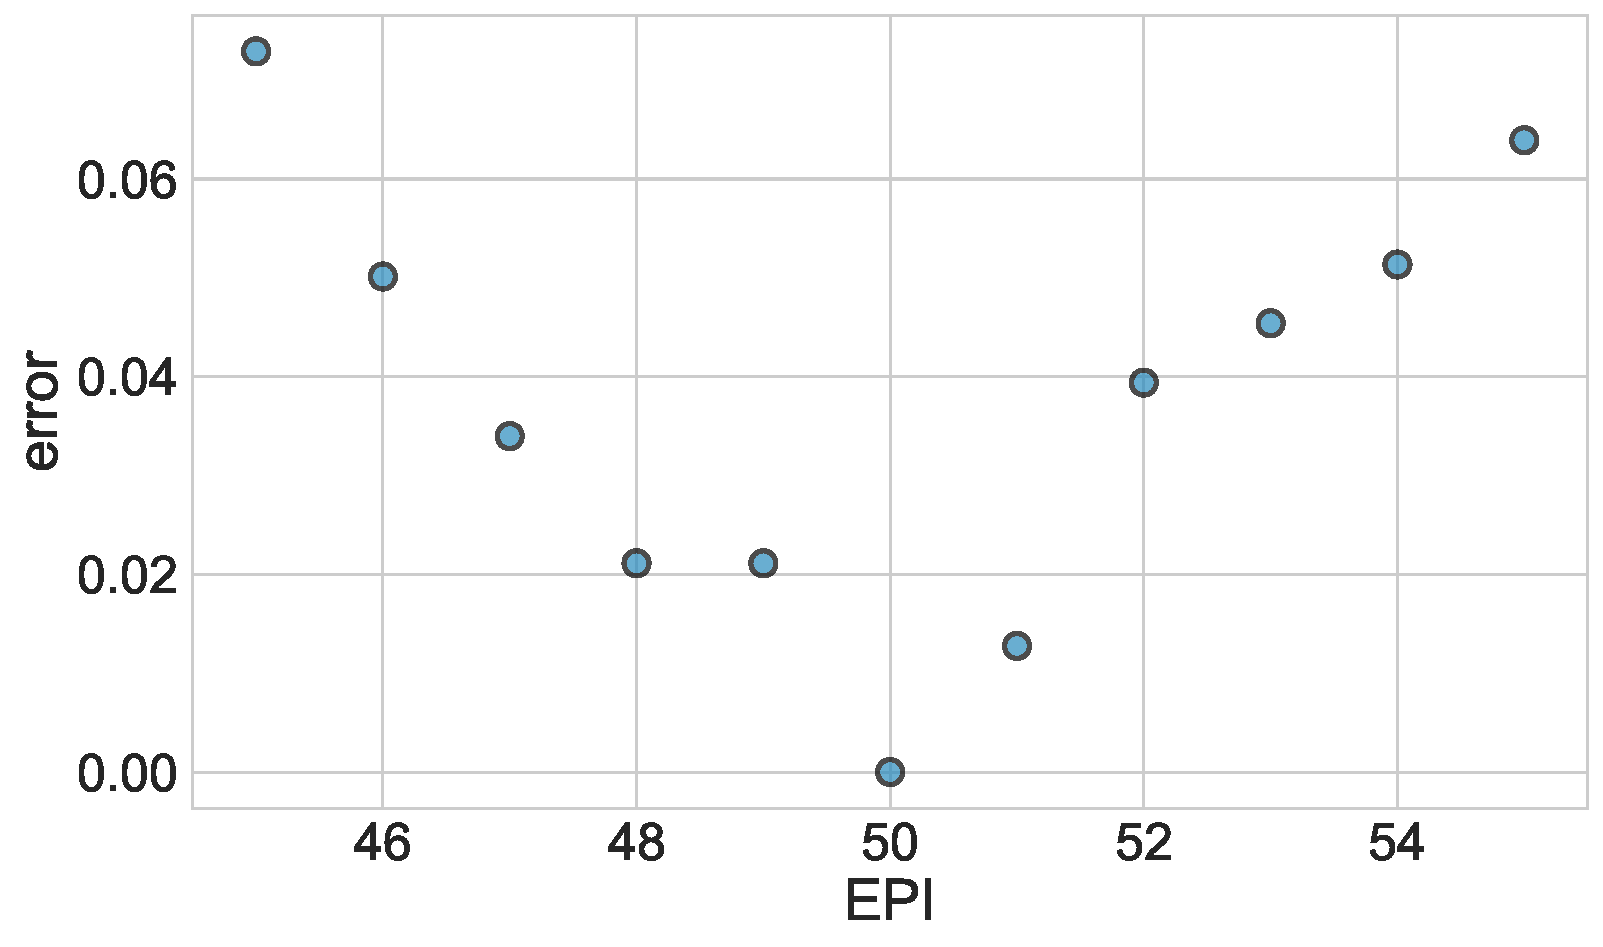
\includegraphics[width=.4\linewidth]{figs/error_EPI}
        \label{fig:exp:future:gdp}
    }
    \subfigure[Sensitivity against FSI]{
        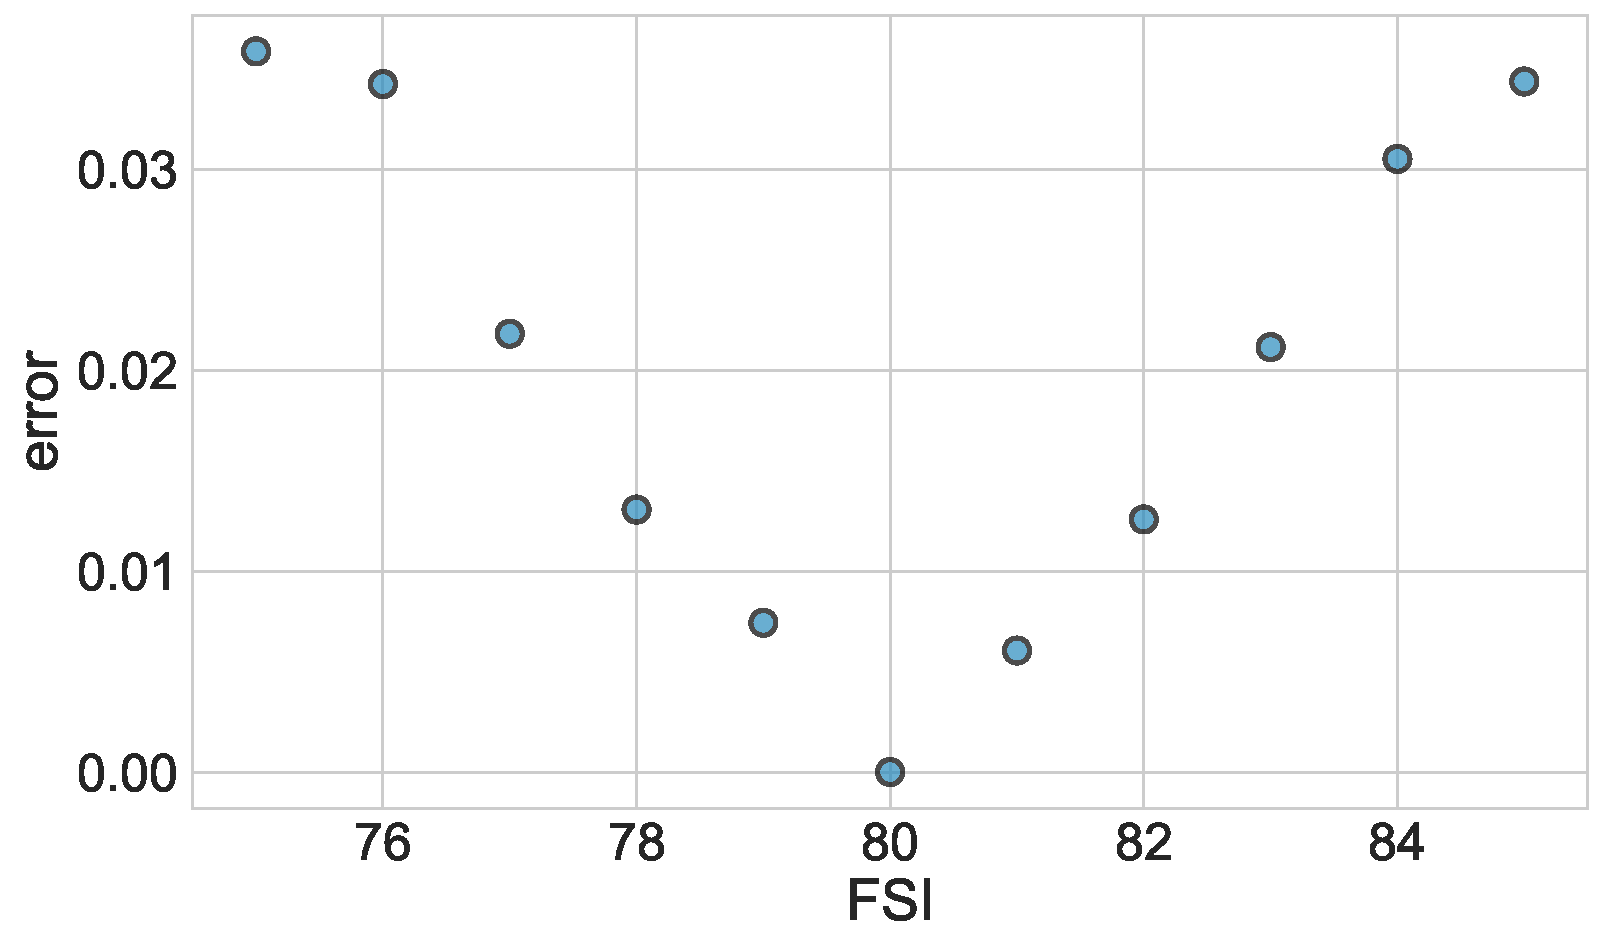
\includegraphics[width=.4\linewidth]{figs/error_FSI}
        \label{fig:exp:future:epi}
    }
    \caption{Fragility Sensitivity Analysis}
    \label{fig:exp:future}
\end{figure}
   \item[2.] \textbf{Predicted model sensitivity analysis}

Here we choose one country (Mauritius), the impact of the direct and indirect effects on the national fragile index are integrated. It is observed that there will not be a significant change in the predicted fragility when the EPI of the environmental index changes.
\begin{figure}[htbp]
    \centering
    \subfigure[Predicted Fragility Sensitivity Analysis]{
        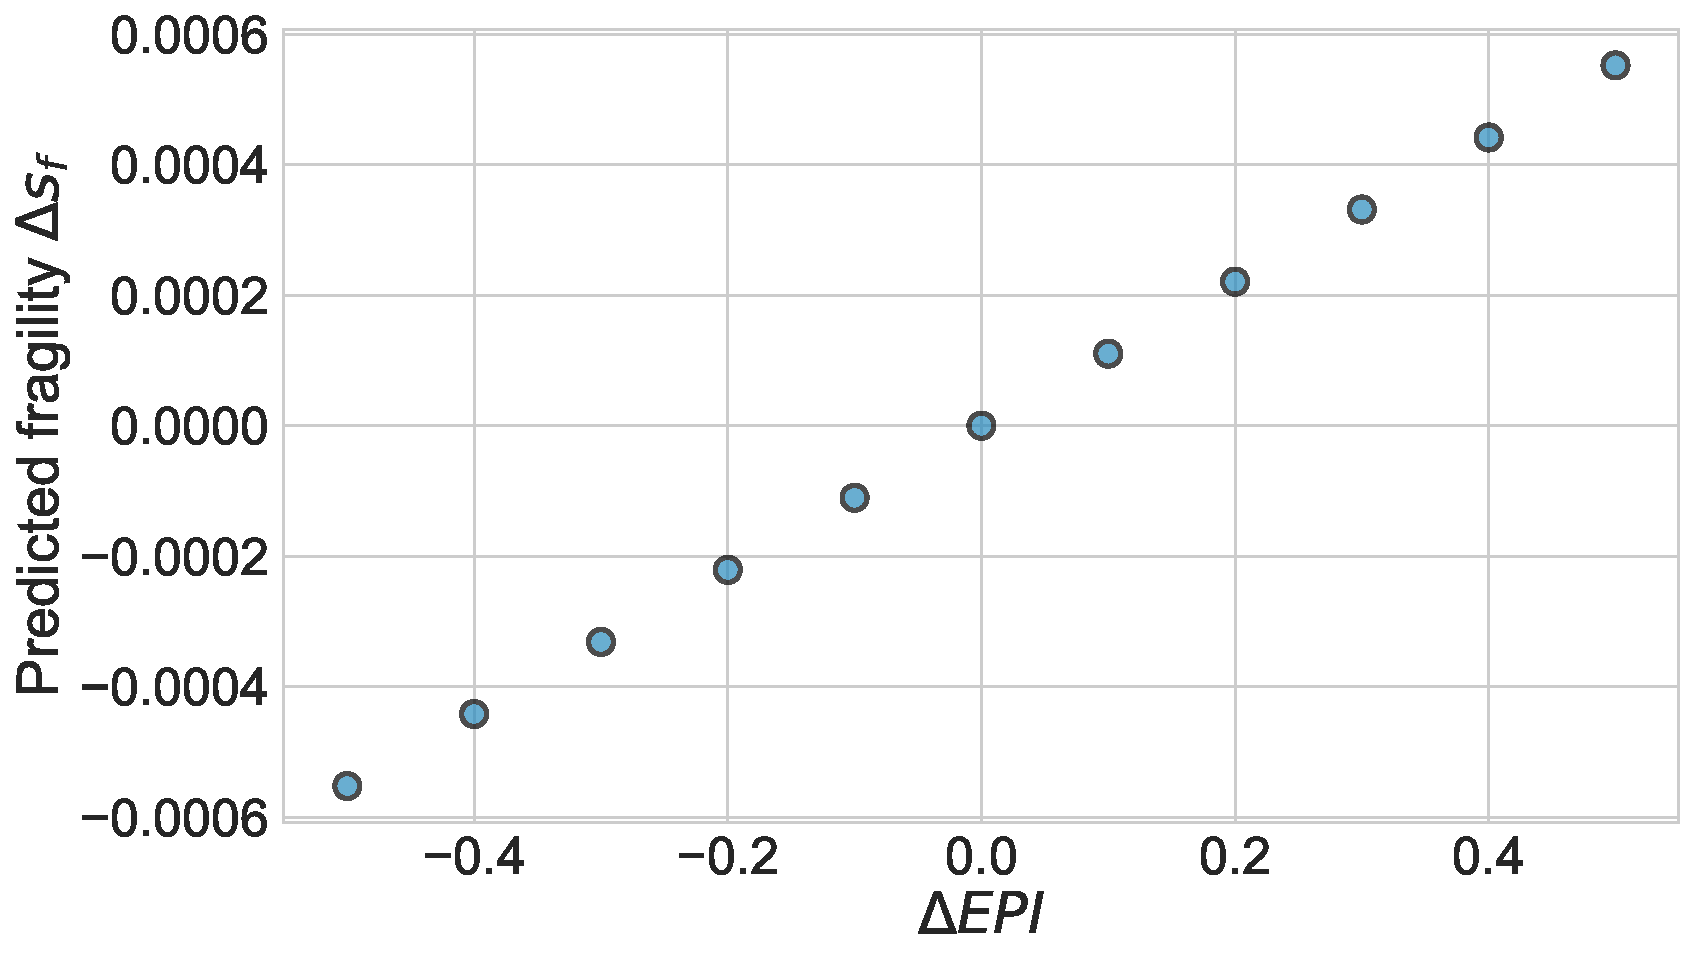
\includegraphics[width=.4\linewidth]{figs/predicted}
        \label{fig:exp:future:gdp}
    }
    \subfigure[Cross Validation]{
        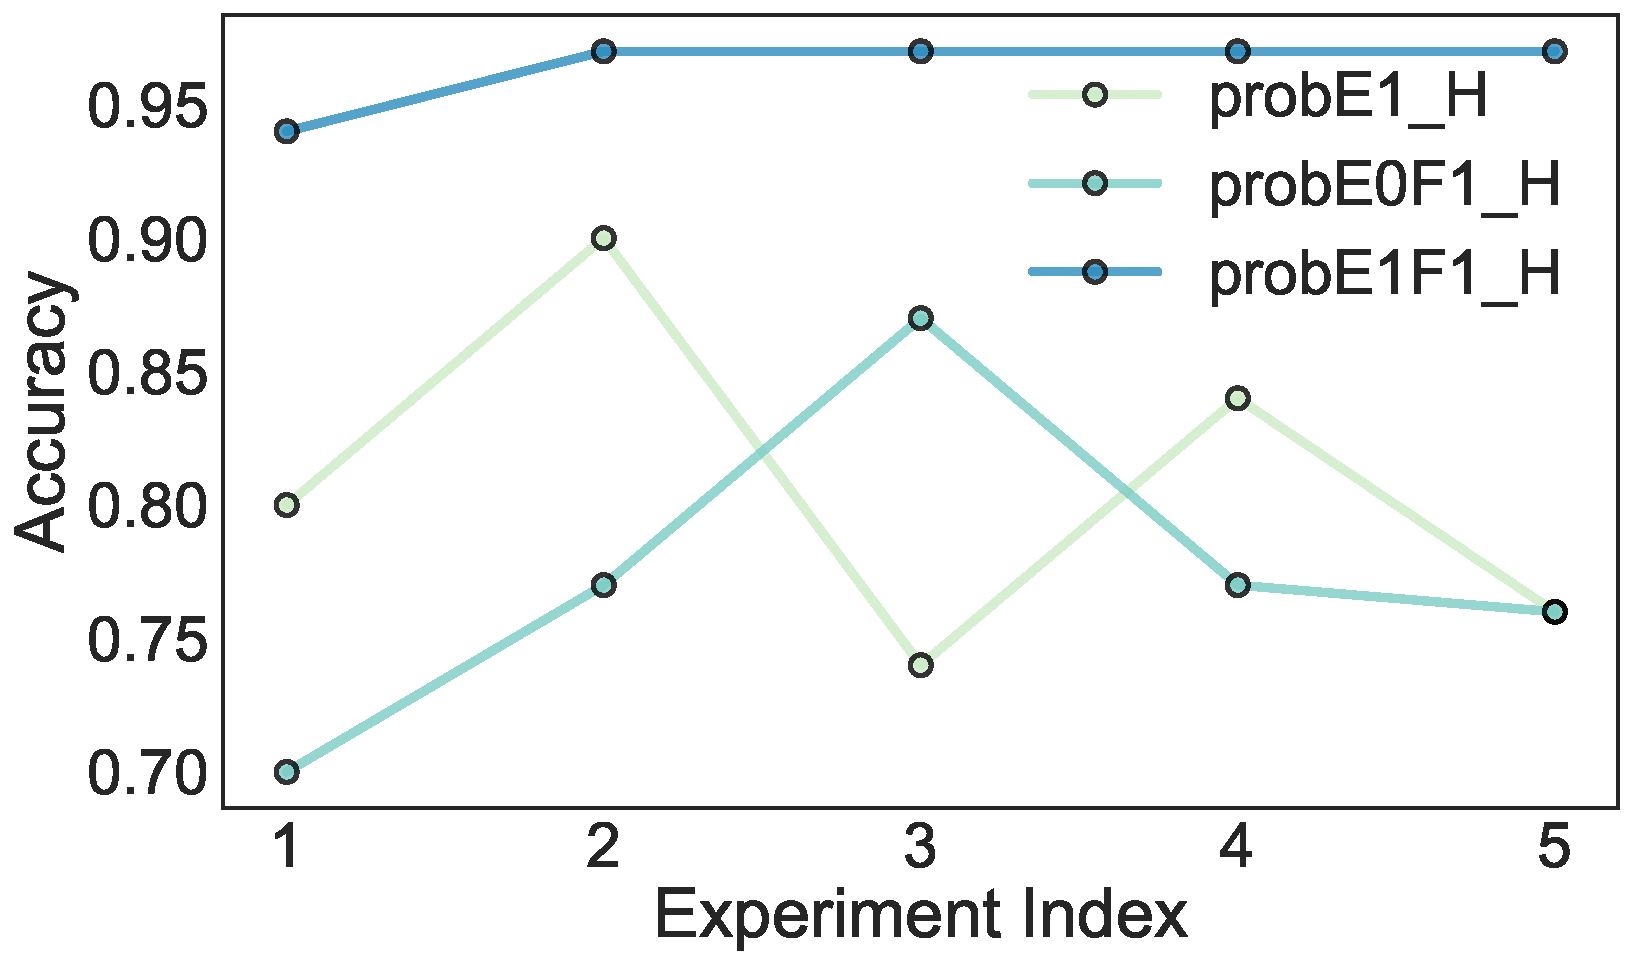
\includegraphics[width=.4\linewidth]{figs/cross_validation}
        \label{fig:exp:future:epi}
    }
    \caption{Sensitivity Analysis}
    \label{fig:exp:future}
\end{figure}
   
   \item[3.] \textbf{Cross-validation for logistic regression}

When calculating the fragility, we use logistic regression to estimate probability. Here we test the accuracy of logistic regression with 5-fold cross-validation. The regression accuracy of different probability varies as the figure shows:
\end{itemize}

\subsection{Strength and Weakness}
We first give overall strength and weakness for our entire framework:
\begin{itemize}
   \item \textbf{Simplicity}. Our model is dedicated to capture the interaction between human and environmental factors in a simple, explainable, and verifiable fasion.
   \item \textbf{Objective}. Basic ideas are derived from convincing facts, while tools used to implement our ideas are theoretically well supported. Human error can be reduced to minimum. 
   \item \textbf{Flexibility}. Our theoretical framework applies to many scenarios other than countries and can be implemented in various methods. 
   \item \textbf{Appealing Results}. The result of our statistical analysis yields concrete conclusions consistent with interdisciplinary facts. The simulation results are convincing and insightful in finding the trade-off between fast economic growth and environment.
\end{itemize}

However, there are plenty of rooms for improvement for our model. 
\begin{itemize}
   \item Some hypothesis are too ideal. For example, we assumed that GDP is representative of human factors in the temporal model, and that EPI represents environmental fragility, without modeling the complex dynamics of climate change.
   \item Data limitation. Our simulation suffers from insufficient amount of data.
   \item Insufficient long-term prediction. Our long-term prediction of GDP and EPI used only recent information of a particular state and cannot well recognize complex dynamics in the long run.
\end{itemize}

\subsection{Extending the Model}

For smaller "states" such as cities, our theoretical framework still applies.
However, specific data preparation, variable selection, and model implementation should be modified accordingly. 
For larger "states" such as continents, our model is in need of describing the interactive relationship between countries to capture the evolution of the climate change and fragility of a organized whole, and its effect on each individual component state.

We give some analysis as follows:
\begin{itemize}
\item	External Intervention: 
It is one of elements given in the FSI index, which in turn plays an important role in our model. Here if we apply our model to figure out issues in terms of regions of various "scale", there is no doubt that its influences will be significantly different. For example, cities of a country must have a closely connection with each other, while continents are not likely to be the same, or certainly not "that closely".
One way to solve this problem is that we can set some systematic measures to represent it. Actually, we can even take it out to discuss its impact with FSI and EPI if necessary.
\item	Different Functions of Cities and National Conditions:
This is especially required to be considered when our model is applied to smaller "states". Different Functions of cities means that fragility is not simply evaluated based on some indexes when it comes to smaller "states" issues. Instead, we are supposed to think over its function in this country. For example, some cities with better economy development or important political status may still not fragile although they have a terrible environment. Besides, different national condition will also affect the model, like different powers of government in every country.
To propose a better model, we may need to cluster different regions and describe the connection in every region more reasonably.
\item	Internal Difference of Continents:
Continents, to the contrary, are so few that there is little variety all over the world. However, if we would like to tell which continent is more fragile, it is necessary to distinguish its internal difference. For example, the fragility of different regions in Asia probably range a lot.
\end{itemize}

\hide{
As we analyzed above, our model requires to include a part to define what is the fragility of a large state, how it varies in different regions and how it influences the evaluation.
}

\subsection{Relation to Environmental Science}

\hide{
An Abrupt Climate Change Scenario and Its Implications for United States National Security (Peter Schwartz et al. 2003)
Is Climate Change a Driver of Armed Conflict? (Ole Magnus Theisen et al. 2013)
Modeling Environmental Security in Sub-Saharan Africa (Amy Richmond Krakowka et al. 2012)
}


Peter Schwartz et al. \cite{schwartz2003abrupt} created an abrupt climate change scenario and analyzed its influence on United States National Security. Although its imagine was reasonable and meaningful for US society, the model was a little simple considering that it was one of pioneer works focusing on environmental security. Instead, our model pay more attention on the relation among human factors, environmental factors and fragility of states.

Like the former work, Ole Magnus Theisen et al. \cite{theisen2013climate} did research on the history of climate change and conflict occurrence. It contributed to linking climate change to conflict, and its methodology of linking elements is similar to our studies of correlation among independent factors. However, our model is interested in the whole framework of relation rather than some concrete climate changes.

Amy Richmond Krakowka et al. \cite{krakowka2012modeling} revealed the environmental security model in an Africa scenario. Its model mainly came from the relation among environment, security and conflict. With a process-outcome framework, it derived a specific conflict analysis, but our model concentrate on the global situation. Besides, we also consider the temporal model. In the process, we figure out how to take measures for the trade-off between economy development and environment protection.

\section{Conclusion}
\label{sec:conclusion}



\bibliography{mybibtex}



\begin{appendices}

\end{appendices}
\end{document}

%% 
%% This work consists of these files mcmthesis.dtx,
%%                                   figures/ and
%%                                   code/,
%% and the derived files             mcmthesis.cls,
%%                                   mcmthesis-demo.tex,
%%                                   README,
%%                                   LICENSE,
%%                                   mcmthesis.pdf and
%%                                   mcmthesis-demo.pdf.
%%
%% End of file `mcmthesis-demo.tex'.

